\chapter{氧化还原平衡与能斯特方程}\label{ch:b1:nernst}

取一根锌片浸入硫酸锌溶液中，另取一根铜片浸入
硫酸铜（Ⅱ）溶液中，用\omterm{def:b1:nernst:cell}{盐桥}连接两种溶液，
再用导线经一只发光二极管把两块金属相连：二极管亮了。
锌与铜离子的反应在单个烧杯中只能使溶液升温，
如今却驱动电子流过导线。
电池就是这一装置的封装形式；pH 计与氯
电极则是它的测量“近亲”。本章使电子交换定量化：
用\omterm{def:b1:nernst:oxidation-number}{氧化数}计数电子，
用\omterm{def:b1:nernst:electrode-potential}{电极电势}给各电对排序，再用\omterm{thm:b1:nernst:nernst}{能斯特方程}
结合浓度追踪它们的变化。

\begin{recall}
第 1 册（十一、十二年级）已定义\omterm{def:b1:nernst:couple}{氧化剂}与\omterm{def:b1:nernst:couple}{还原剂}，
写出\omterm{def:b1:nernst:couple}{半反应式}，用两种金属和两种溶液组装电池，
并把锌–铜电池视为一种电池。\omterm{def:b1:extent-q-and-k:quotient}{反应商}
与平衡常数均取自\cref{ch:b1:extent-q-and-k}；
溶质的\omterm{def:b1:extent-q-and-k:activity}{活度}为 $c/c^\circ$，气体的为 $p/p^\circ$，
纯固体与纯液体的为 1。
\end{recall}

\section{氧化数与电对}

\begin{definition}[氧化剂、还原剂、氧化还原电对、半反应式]\label{def:b1:nernst:couple}
能够得到电子的物种称为\emph{氧化剂}\index{氧化剂}，
能够给出电子的物种称为\emph{还原剂}\index{还原剂}。氧化剂 Ox 与它所转化成的还原剂 Red
构成\emph{氧化还原
电对}\index{氧化还原电对} Ox/Red，可由其
\emph{半反应式}\index{半反应式}表示为
$\alpha\,\mathrm{Ox} + n\,\mathrm{e^-} \rightleftharpoons
\beta\,\mathrm{Red}$，原子须配平，必要时用 \ce{H2O} 与 \ce{H+}，
电荷则用电子配平。
\end{definition}

氧化还原反应是两个电对之间的电子交换：一个电对的
\omterm{def:b1:nernst:couple}{氧化剂}被还原，另一电对的\omterm{def:b1:nernst:couple}{还原剂}被氧化，
两者的电子恰好抵消。要数清复杂物种中的电子，需为每个
原子指定一个\omterm{def:b1:nernst:oxidation-number}{氧化数}。

\begin{definition}[氧化数]\label{def:b1:nernst:oxidation-number}
物种中某原子的\emph{氧化数}\index{氧化数}，
是指若断开全部化学键，并将每对成键电子全部归于\omterm{def:b1:periodicity:electronegativity}{电负性}较大的原子时，该原子所带的
电荷（两个相同原子之间的\omterm{def:b1:lewis-resonance-vsepr:lewis}{成键电子对}则平分），
书写时用罗马数字，如铁（Ⅲ）、
高锰酸根离子中的 \ce{Mn^{+VII}}。
\end{definition}

\begin{proposition}[氧化数的规则]\label{prop:b1:nernst:on-rules}
\begin{enumerate}
  \item 单质中的原子\omterm{def:b1:nernst:oxidation-number}{氧化数}为 0；单原子离子的
        其电荷。
  \item 物种中各原子的\omterm{def:b1:nernst:oxidation-number}{氧化数}之和等于其
        电荷。
  \item 氢的\omterm{def:b1:nernst:oxidation-number}{氧化数}为 $+$I（在金属氢化物中为 $-$I）；氧的
        \omterm{def:b1:nernst:oxidation-number}{氧化数}为 $-$II（在过氧化物中为 $-$I，与氟成键时除外）；氟的
        \omterm{def:b1:nernst:oxidation-number}{氧化数}为 $-$I。
  \item \omterm{def:b1:nernst:couple}{半反应式}中的电子数等于发生变化的元素
        的\omterm{def:b1:nernst:oxidation-number}{氧化数}变化量乘以
        其原子个数。
\end{enumerate}
\end{proposition}

\begin{proof}
1 与 2：断开全部化学键时电荷守恒，相同原子之间
不发生电子转移。3：氢的\omterm{def:b1:periodicity:electronegativity}{电负性}小于与之成键的每一种
非金属（见\cref{ch:b1:periodicity}），并大于碱
金属；氧的\omterm{def:b1:periodicity:electronegativity}{电负性}大于除氟外的所有元素，
在 \ce{O-O} 中共用电子对被平分。4：H 与 O 的\omterm{def:b1:nernst:oxidation-number}{氧化数}保持不变，
因此\omterm{def:b1:lewis-resonance-vsepr:formal-charge}{形式电荷}发生变化的原子只有
相关元素的原子，而电子在\omterm{def:b1:nernst:couple}{半反应式}中出现的数目恰好用以
配平这一电荷变化。
\end{proof}

\begin{method}[物种的氧化数]\label{met:b1:nernst:oxidation-numbers}
按惯例给 H、O、F 及离子赋以常见\omterm{def:b1:nernst:oxidation-number}{氧化数}，其余原子的
\omterm{def:b1:nernst:oxidation-number}{氧化数}由规则 2 得出。在 \ce{MnO4-} 中：$x + 4(-2) = -1$，$x = +7$。
在 \ce{Cr2O7^2-} 中：$2x - 14 = -2$，$x = +6$。在 \ce{S4O6^2-} 中，平均
\omterm{def:b1:nernst:oxidation-number}{氧化数}为 $+2.5$；\omterm{def:b1:lewis-resonance-vsepr:lewis}{路易斯结构}显示硫有两种。
\end{method}

\begin{method}[配平半反应式]\label{met:b1:nernst:balance-by-on}
\begin{enumerate}
  \item 配平\omterm{def:b1:nernst:oxidation-number}{氧化数}发生变化的元素。
  \item 添加电子：\omterm{def:b1:nernst:oxidation-number}{氧化数}的变化量乘以
        原子个数。
  \item 用 \ce{H+}（酸性溶液）或 \ce{OH-}
        （碱性溶液）配平电荷。
  \item 用 \ce{H2O} 配平氢和氧，最后核对氧。
\end{enumerate}
对酸性溶液中的高锰酸根离子：Mn 由 $+$VII 变为 $+$II，故需 5
个电子；左边电荷为 $-1 - 5 = -6$，右边为 $+2$，
故需 $8\,\ce{H+}$；再加 $4\,\ce{H2O}$：
\ce{MnO4- + 8H+ + 5e- -> Mn^2+ + 4H2O}.
\end{method}

\section{电化学电池}

\begin{definition}[电化学电池]\label{def:b1:nernst:cell}
\emph{电化学电池}\index{电化学电池}是由两个
\emph{半电池}\index{半电池}通过离子导体相连构成的装置，每个半电池由一个电对与一个
电子导体（即电极）组成，离子导体常为
\emph{盐桥}\index{盐桥}（由浓的惰性盐，
如硝酸钾，制成的凝胶或管）。发生氧化的电极称为
\emph{阳极}\index{阳极}，发生还原的电极称为
\emph{阴极}\index{阴极}。\emph{电池
电压}\index{电池电压}是两电极之间的电势差，
即正极电势减负极电势，在
无电流通过时测得。
\end{definition}

\begin{omfigure}
\begin{tikzpicture}[font=\small, >={Stealth}]
  \pic at (0,0) {beaker={0.7}{omDef!14}};
  \pic at (3.6,0) {beaker={0.7}{omDef!32}};
  \pic at (-0.3,0.25) {electrode={black!35}};
  \pic at (3.9,0.25) {electrode={orange!70!brown}};
  \pic at (0.35,0.55) {saltbridge={2.9}};
  \pic (m) at (1.8,4.3) {meter={V}};
  \draw[thick] (-0.15,2.65) |- (m-a);
  \draw[thick] (4.05,2.65) |- (m-b);
  \node[anchor=east] at (-0.95,1.0) {\ce{Zn}};
  \node[anchor=west] at (4.45,1.0) {\ce{Cu}};
  \node at (0.25,-0.35) {\ce{Zn^2+}, \ce{SO4^2-}};
  \node at (3.6,-0.35) {\ce{Cu^2+}, \ce{SO4^2-}};
  \draw[->, omProp, thick] (-0.15,3.35) -- (0.8,3.35) node[above, midway] {$\mathrm{e^-}$};
  \draw[->, omProp, thick] (2.8,3.35) -- (3.75,3.35) node[above, midway] {$\mathrm{e^-}$};
  \node[anchor=east] at (-0.9,2.3) {$-$ 阳极};
  \node[anchor=west] at (4.6,2.3) {阴极 $+$};
  \node[font=\scriptsize, align=center] at (1.8,2.75) {盐桥 \\ \ce{K+} $\rightarrow$ \quad $\leftarrow$ \ce{NO3-}};
  \node[font=\scriptsize] at (-0.1,-0.8) {\ce{Zn -> Zn^2+ + 2e-}};
  \node[font=\scriptsize] at (3.7,-0.8) {\ce{Cu^2+ + 2e- -> Cu}};
\end{tikzpicture}

{\small 锌–铜（丹尼尔）电池。锌在\omterm{def:b1:nernst:cell}{阳极}被氧化，\omterm{def:b1:nernst:cell}{阳极}为负极；
铜离子在\omterm{def:b1:nernst:cell}{阴极}被还原，\omterm{def:b1:nernst:cell}{阴极}为正极。
电子经外电路由锌流向铜；
在\omterm{def:b1:nernst:cell}{盐桥}中，阳离子向\omterm{def:b1:nernst:cell}{阴极}迁移，阴离子向\omterm{def:b1:nernst:cell}{阳极}迁移，
从而使两个溶液均保持电中性。}
\end{omfigure}

将电池写成一条线，\omterm{def:b1:nernst:cell}{阳极}写在左侧：\ce{Zn} $|$ \ce{Zn^2+}
$\|$ \ce{Cu^2+} $|$ \ce{Cu}，单竖线表示相界面，双竖线表示\omterm{def:b1:nernst:cell}{盐桥}。
所有浓度均为 \qty{1}{mol/L} 时，
电池的电压为 \qty{1.10}{V}。电池供出电流时发生的反应为
\ce{Zn + Cu^2+ -> Zn^2+ + Cu}，它正是在单一烧杯中会发生的反应；
将两个\omterm{def:b1:nernst:cell}{半电池}分开后，电子被迫经导线流动，
从而能够做功。

\section{电极电势}

电压是一个差值：只有两个\omterm{def:b1:nernst:cell}{半电池}之间的电势差才能被测量。
因此，参比\omterm{def:b1:nernst:cell}{半电池}需要一次性选定。

\begin{definition}[电极电势，标准电极电势]\label{def:b1:nernst:electrode-potential}
\emph{标准氢电极}\index{标准氢电极}是一个铂电极，
与压强为 \qty{1}{bar} 的氢气接触，并
浸入 \ce{H+} \omterm{def:b1:extent-q-and-k:activity}{活度}为 1 的理想溶液中。\omterm{def:b1:nernst:cell}{半电池}的
\emph{电极电势}\index{电极电势} $E$ 为\omterm{def:b1:nernst:cell}{半电池}的电压，
即以标准氢电极为左侧构成的电池的电压：
$E = V_{\text{半电池}} - V_{\text{SHE}}$。当电对的每种物质\omterm{def:b1:extent-q-and-k:activity}{活度}均为 1 时，
此电势即为该电对的\emph{标准电极电势}\index{标准电极电势}
$E^\circ$，在给定温度下为定值。
\end{definition}

\begin{omfigure}
\begin{tikzpicture}[font=\small, >={Stealth}]
  \pic at (0,0) {beaker={0.72}{omDef!14}};
  % glass jacket, open at the bottom, with the gas inlet on the right
  \draw[om glass] (-0.32,0.35) -- (-0.32,3.0) -- (0.32,3.0) -- (0.32,2.55)
    -- (0.95,2.55) (0.32,2.35) -- (0.95,2.35) (0.32,2.35) -- (0.32,0.35);
  \draw[thick] (0,0.9) -- (0,3.45);
  \fill[black!60] (-0.16,0.5) rectangle (0.16,0.9);
  \foreach \x/\y in {0.45/0.45, 0.55/0.75, 0.48/1.05, -0.45/0.5, -0.52/0.85}
    \draw[omDef!70] (\x,\y) circle (0.055);
  \draw[->] (1.9,2.45) node[right] {\ce{H2}, \qty{1}{bar}} -- (1.0,2.45);
  \draw (0.12,0.7) -- (1.5,0.2) node[right] {镀铂的铂};
  \draw (-0.6,1.1) -- (-1.4,1.6) node[left] {\ce{H+}，活度为 1};
  \node[anchor=west] at (0.05,3.45) {接至电路};
\end{tikzpicture}

{\small \omterm{def:b1:nernst:electrode-potential}{标准氢电极}：氢气鼓泡通过表面覆有细铂的铂片，
铂片浸入 \ce{H+} \omterm{def:b1:extent-q-and-k:activity}{活度}为 1 的溶液中。
其电对为 \ce{H+}/\ce{H2}，按
约定其电势为 0。}
\end{omfigure}

氢电极使用起来不太方便，实验室通常
改用另一种更便利、电势已知的\omterm{def:b1:nernst:cell}{半电池}进行测量。

\begin{definition}[参比电极]\label{def:b1:nernst:reference-electrode}
\emph{参比电极}\index{参比电极}是一种电势固定且已知的\omterm{def:b1:nernst:cell}{半电池}，
例如银–氯化银电极（银丝表面包覆氯化银，
浸于浓度固定的氯化物溶液中）；
或甘汞电极（汞
与 \ce{Hg2Cl2} 及氯化物溶液接触）。
\end{definition}

下表给出本册所用的\omterm{def:b1:nernst:electrode-potential}{标准电极电势}；
下一节的竖直标尺给出了其中最常见的几种。

\begin{omfigure}
\begin{tabular}{lr@{\qquad}lr}
\hline
电对 & $E^\circ$ (V) & 电对 & $E^\circ$ (V) \\
\hline
\ce{Li+}/\ce{Li} & $-3.04$ & \ce{Cu^2+}/\ce{Cu} & 0.34 \\
\ce{K+}/\ce{K} & $-2.94$ & $[\ce{Fe(CN)6}]^{3-}$/$[\ce{Fe(CN)6}]^{4-}$ & 0.36 \\
\ce{Na+}/\ce{Na} & $-2.71$ & \ce{Cu+}/\ce{Cu} & 0.52 \\
\ce{Mg^2+}/\ce{Mg} & $-2.36$ & \ce{I2}/\ce{I-} & 0.53 \\
\ce{Al^3+}/\ce{Al} & $-1.68$ & \ce{O2}/\ce{H2O2} & 0.69 \\
\ce{Zn^2+}/\ce{Zn} & $-0.76$ & \ce{Fe^3+}/\ce{Fe^2+} & 0.77 \\
\ce{Fe^2+}/\ce{Fe} & $-0.41$ & \ce{Hg2^2+}/\ce{Hg} & 0.80 \\
\ce{Ni^2+}/\ce{Ni} & $-0.24$ & \ce{Ag+}/\ce{Ag} & 0.80 \\
\ce{Pb^2+}/\ce{Pb} & $-0.13$ & \ce{Br2}/\ce{Br-} & 1.08 \\
\ce{H+}/\ce{H2} & 0 & \ce{O2}/\ce{H2O} & 1.23 \\
\ce{S4O6^2-}/\ce{S2O3^2-} & 0.02 & \ce{MnO2}/\ce{Mn^2+} & 1.23 \\
\ce{Cu^2+}/\ce{Cu+} & 0.16 & \ce{Cl2}/\ce{Cl-} & 1.36 \\
\ce{AgCl}/\ce{Ag} & 0.22 & \ce{PbO2}/\ce{Pb^2+} & 1.46 \\
\ce{Hg2Cl2}/\ce{Hg} & 0.27 & \ce{MnO4-}/\ce{Mn^2+} & 1.51 \\
 & & \ce{HClO}/\ce{Cl2} & 1.63 \\
 & & \ce{H2O2}/\ce{H2O} & 1.76 \\
\hline
\end{tabular}

\smallskip
{\small 在 \qty{25}{\celsius} 下，\omterm{def:b1:nernst:electrode-potential}{标准电极电势}由各电对中物种的
表列标准吉布斯生成能计算得到。
与其他汇编数据相比，数值可能相差
几百分之几伏。}
% ledger: dfg:Li+_ao, dfg:K+_ao, dfg:Na+_ao, dfg:Mg2+_ao, dfg:Al3+_ao, dfg:Zn2+_ao, dfg:Fe2+_ao, dfg:Ni2+_ao, dfg:Pb2+_ao (computed in figdata/bachelor-1/standard-potentials.py)
% ledger: dfg:S4O62-_ao, dfg:S2O32-_ao, dfg:Cu2+_ao, dfg:Cu+_ao, dfg:AgCl_cr, dfg:Cl-_ao, dfg:Hg2Cl2_cr, dfg:Fe_CN63-_ao, dfg:Fe_CN64-_ao, dfg:I-_ao (same script)
% ledger: dfg:H2O2_ao, dfg:Fe3+_ao, dfg:Hg22+_ao, dfg:Ag+_ao, dfg:Br-_ao, dfg:H2O_l, dfg:MnO2_cr, dfg:Mn2+_ao, dfg:PbO2_cr, dfg:MnO4-_ao, dfg:HClO_ao (same script)
\end{omfigure}

\section{能斯特方程}

\begin{theorem}[能斯特方程]\label{thm:b1:nernst:nernst}
对于电对 $\alpha\,\text{氧化态} + n\,\mathrm{e^-} \rightleftharpoons
\beta\,\text{还原态}$，两侧还可能含有其他物种（\ce{H+}、\ce{H2O}、
\ce{Cl-}）位于任一侧，则\omterm{def:b1:nernst:electrode-potential}{电极电势}由
\emph{能斯特方程}\index{能斯特方程}给出
\[
  E = E^\circ + \frac{RT}{nF}\ln\frac{\prod a_{\text{氧化侧}}^{\nu}}{\prod
  a_{\text{还原侧}}^{\nu}}
  = E^\circ + \frac{0.059}{n}\log\frac{a(\text{氧化态})^\alpha\,\cdots}{a(\text{还原态})^\beta\,\cdots}
  \quad\text{在 \qty{25}{\celsius} 下},
\]
其中每个\omterm{def:b1:extent-q-and-k:activity}{活度}都带有其\omterm{def:b1:extent-q-and-k:extent}{化学计量数}，因子
$RT\ln 10/F = \qty{0.059}{V}$ 在 \qty{298}{K} 时取值。
\end{theorem}

\admitted{\omterm{thm:b1:nernst:nernst}{能斯特方程}由反应的吉布斯能与\omterm{def:b1:nernst:cell}{电池电压}之间的关系导出，
该关系见于本科二年级
分册。}

\begin{example}[三个电对]\label{ex:b1:nernst:examples}
\ce{Cu^2+}/\ce{Cu}：$E = 0.34 + 0.030\log[\ce{Cu^2+}]$（金属铜
的\omterm{def:b1:extent-q-and-k:activity}{活度}为 1）。
\ce{Fe^3+}/\ce{Fe^2+}：$E = 0.77 + 0.059\log([\ce{Fe^3+}]/[\ce{Fe^2+}])$。
\ce{MnO4-}/\ce{Mn^2+}：$E = 1.51 + \frac{0.059}{5}\log
\frac{[\ce{MnO4-}][\ce{H+}]^8}{[\ce{Mn^2+}]}$；当高锰酸根与锰（II）
的浓度相等时，$E = 1.51 - 0.094\,\mathrm{pH}$：
高锰酸根的氧化能力随 pH 升高而下降。
\end{example}

浓度变化十倍，电势改变 $0.059/n$
伏，即几十毫伏量级。因此，测得精确到毫伏的电压
是浓度的准确量度，这正是 pH 电极的原理，
也是周末问题中氯电极的原理。

\begin{history}[瓦尔特·能斯特]
\begin{minipage}[t]{0.22\linewidth}\vspace{0pt}
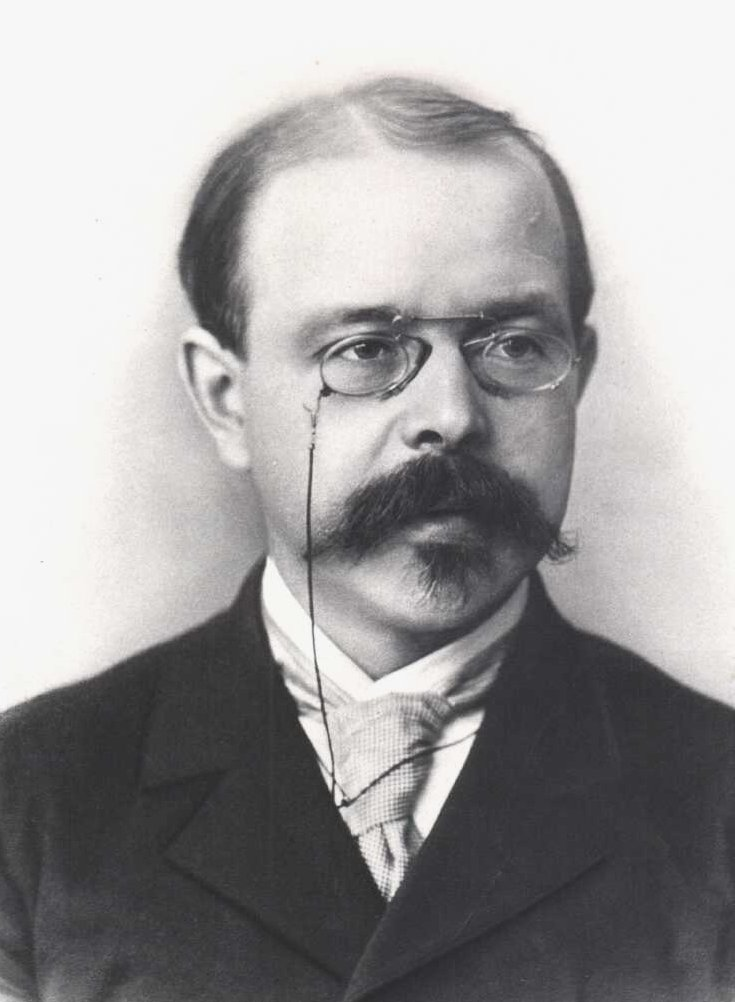
\includegraphics[width=\linewidth]{images/book2/nernst.jpg}
\end{minipage}\hfill
\begin{minipage}[t]{0.74\linewidth}\vspace{0pt}
瓦尔特·能斯特（1864--1941），摄于 1889 年，时年二十五岁。本节的方程
将\omterm{def:b1:nernst:cell}{电池电压}与其离子的浓度联系起来，
以他的名字命名；热力学第三定律也以他的名字命名，
该定律见于本科二年级分册。
（照片：Smithsonian Libraries，公有领域，维基共享资源。）
\end{minipage}
\end{history}

\section{预测氧化还原反应}

\begin{method}[预测氧化还原反应]\label{met:b1:nernst:predict-redox}
\begin{enumerate}
  \item 将各电对按\omterm{def:b1:nernst:electrode-potential}{标准电极电势}排列在竖直刻度上，
        \omterm{def:b1:nernst:couple}{氧化剂}在左，\omterm{def:b1:nernst:couple}{还原剂}在右。
  \item 存在的最强\omterm{def:b1:nernst:couple}{氧化剂}（$E^\circ$ 最高）与
        存在的最强\omterm{def:b1:nernst:couple}{还原剂}（$E^\circ$ 最低）发生反应：箭头由
        \omterm{def:b1:nernst:couple}{氧化剂}向下指向\omterm{def:b1:nernst:couple}{还原剂}，再向上指向生成物，
        形成一个希腊字母 $\gamma$。
  \item 当\omterm{def:b1:nernst:couple}{氧化剂}电对位于\omterm{def:b1:nernst:couple}{还原剂}电对之上时，反应有利（$K > 1$）；
        实际中，若两者电势之差
        超过约 \qty{0.25}{V}（每交换一个电子），则可视为\omterm{def:b1:extent-q-and-k:quantitative}{定量反应}。
\end{enumerate}
\end{method}

\begin{omfigure}
\begin{tikzpicture}[font=\small, >={Stealth}, y=2.6cm]
  \draw[->, thick] (0,-1.0) -- (0,1.85) node[above] {$E^\circ$ (V)};
  \foreach \e/\o/\r in {-0.76/\ce{Zn^2+}/\ce{Zn}, 0/\ce{H+}/\ce{H2},
      0.34/\ce{Cu^2+}/\ce{Cu}, 0.77/\ce{Fe^3+}/\ce{Fe^2+},
      1.36/\ce{Cl2}/\ce{Cl-}, 1.51/\ce{MnO4-}/\ce{Mn^2+}} {
    \draw (-0.12,\e) -- (0.12,\e);
    \node[anchor=east] at (-0.25,\e) {\o};
    \node[anchor=west] at (0.25,\e) {\r};
    \node[anchor=west, black!55, font=\scriptsize] at (2.0,\e) {\e};
  }
  \node[omProp] at (-1.0,1.85) {氧化剂};
  \node[omDef] at (1.1,1.85) {还原剂};
  % the gamma: Cu2+ meets Zn below it on the other side
  \draw[omThm, very thick, ->, rounded corners=4pt] (-1.0,0.28) -- (-1.0,-0.42) -- (0.6,-0.70);
  \draw[omThm, thick, ->] (-0.5,0.40) to[bend left=40] (0.5,0.40);
  \draw[omThm, thick, ->] (0.5,-0.85) to[bend left=40] (-0.5,-0.85);
\end{tikzpicture}

{\small \omterm{def:b1:nernst:electrode-potential}{标准电极电势}示意图。伽马规则：\omterm{def:b1:nernst:couple}{氧化剂}
\ce{Cu^2+} 与另一侧位于其下方的\omterm{def:b1:nernst:couple}{还原剂} \ce{Zn} 发生反应
（粗箭头）；\ce{Cu^2+} 还原为 \ce{Cu}（上方曲线箭头），
\ce{Zn} 氧化为 \ce{Zn^2+}（下方曲线箭头）。逆反应
\ce{Cu} 与 \ce{Zn^2+} 的反应则不利。}
\end{omfigure}

\begin{proposition}[由标准电极电势求平衡常数]\label{prop:b1:nernst:equilibrium-constant}
对于反应 $\text{氧化态1} + \text{还原态2} \rightleftharpoons
\text{还原态1} + \text{氧化态2}$，交换 $n$ 个电子，
\[
  \log K = \frac{n\,(E^\circ_1 - E^\circ_2)}{0.059}\quad\text{在 \qty{25}{\celsius} 下} .
\]
\end{proposition}

\begin{proof}
平衡时，由两电对组成的电池中无电流通过：
两电极的电势相等，$E_1 = E_2$。对每一电对写出\omterm{thm:b1:nernst:nernst}{能斯特方程}
（取相同的 $n$）：$E^\circ_1 + \frac{0.059}{n}\log
\frac{a(\text{氧化态1})}{a(\text{还原态1})} = E^\circ_2 + \frac{0.059}{n}\log
\frac{a(\text{氧化态2})}{a(\text{还原态2})}$，于是 $\frac{n(E^\circ_1 -
E^\circ_2)}{0.059} = \log\frac{a(\text{还原态1})a(\text{氧化态2})}{a(\text{氧化态1})
a(\text{还原态2})} = \log K$，其中\omterm{def:b1:extent-q-and-k:activity}{活度}取平衡时的值。
\end{proof}

对于丹尼尔电池反应，$\log K = 2(0.34 + 0.76)/0.059 = 37$：锌
将铜离子完全还原。对于 \ce{2Fe^3+ + 2I- <=> 2Fe^2+ + I2}，
$\log K = 2(0.77 - 0.53)/0.059 = 8.1$。该方法的判据如下：
取 $n = 1$，若电势差为 \qty{0.25}{V}，则 $K = 10^{4.2}$。

\begin{proposition}[组合电势]\label{prop:b1:nernst:combined-potentials}
若电对 $\mathrm{A}/\mathrm{B}$（转移 $n_1$ 个电子）与
$\mathrm{B}/\mathrm{C}$（$n_2$）组合成 $\mathrm{A}/\mathrm{C}$
（$n_3 = n_1 + n_2$），则 $n_3 E^\circ_3 = n_1 E^\circ_1 + n_2 E^\circ_2$。
电势不可直接相加，而以电子数加权的电势可以相加。
\end{proposition}

\begin{proof}
溶液中含 A、B、C，并与一个电极处于平衡，
此时三个电对的电势相同，均为 $E$。将第一式乘以 $n_1$、第二式乘以 $n_2$，再相加：
B 的\omterm{def:b1:extent-q-and-k:activity}{活度}相消，得 $(n_1 + n_2)E = n_1E^\circ_1 + n_2E^\circ_2 +
0.059\log\frac{a(\mathrm{A})}{a(\mathrm{C})}$，
此即 $n_3$ 倍的 A/C \omterm{thm:b1:nernst:nernst}{能斯特方程}，
其中 $E^\circ_3$ 如所述。
\end{proof}

对于铜：$2E^\circ(\ce{Cu^2+}/\ce{Cu}) = 0.16 + 0.52 = 0.68$，故
$E^\circ(\ce{Cu^2+}/\ce{Cu}) = 0.34$~V，与表中一致。由于
$E^\circ(\ce{Cu+}/\ce{Cu}) > E^\circ(\ce{Cu^2+}/\ce{Cu+})$，亚铜离子
自身发生氧化与还原，\ce{2Cu+ -> Cu^2+ + Cu}：它在水中不能稳定存在
（见\cref{ch:b1:e-ph-diagrams}）。

\begin{proposition}[第二类电极]\label{prop:b1:nernst:second-kind}
表面包覆氯化银的银丝置于氯化物溶液中，
其电势为
\[
  E = E^\circ(\ce{AgCl}/\ce{Ag}) - 0.059\log[\ce{Cl-}], \qquad
  E^\circ(\ce{AgCl}/\ce{Ag}) = E^\circ(\ce{Ag+}/\ce{Ag}) - 0.059\,\mathrm{p}K_s(\ce{AgCl}) .
\]
\end{proposition}

\begin{proof}
银丝与溶液中的 \ce{Ag+} 达到平衡：
$E = E^\circ(\ce{Ag+}/\ce{Ag}) + 0.059\log[\ce{Ag+}]$，而氯化银决定
$[\ce{Ag+}] = K_s/[\ce{Cl-}]$。代入得
$E = E^\circ(\ce{Ag+}/\ce{Ag}) + 0.059\log K_s - 0.059\log[\ce{Cl-}]$。
\end{proof}

数值上 $0.80 - 0.059 \times 9.75 = 0.22$~V，与表中数值一致，
该值由吉布斯自由能独立求得。此类电极
可用于测定氯离子，或在氯离子浓度固定时用作\omterm{def:b1:nernst:reference-electrode}{参比电极}。

\section{练习}

\begin{exercise}[$\star$]\label{exo:b1:nernst:1}
求下列加下划线原子的\omterm{def:b1:nernst:oxidation-number}{氧化数}：\ce{\underline{N}H3}、
\ce{\underline{N}O3-}、\ce{\underline{S}O4^2-}、\ce{H2\underline{O}2}、
\ce{\underline{Cr}2O7^2-}、\ce{\underline{Cl}O-}、\ce{\underline{Fe}3O4}
（取平均值）、\ce{\underline{C}H3OH}。
\end{exercise}

\begin{exercise}[$\star$]\label{exo:b1:nernst:2}
在酸性介质中配平下列\omterm{def:b1:nernst:couple}{半反应式}：\ce{Cr2O7^2-}/\ce{Cr^3+}、
\ce{H2O2}/\ce{H2O}、\ce{O2}/\ce{H2O2} 与 \ce{SO4^2-}/\ce{SO2}。
\end{exercise}

\begin{exercise}[$\star$]\label{exo:b1:nernst:3}
写出 \ce{Zn^2+}/\ce{Zn}、\ce{Cl2}/\ce{Cl-}、
\ce{O2}/\ce{H2O} 与 \ce{Hg2Cl2}/\ce{Hg} 的\omterm{thm:b1:nernst:nernst}{能斯特方程}，并计算
锌片在 \qty{0.010}{mol/L} 硫酸锌溶液中的电势。
\end{exercise}

\begin{exercise}[$\star$]\label{exo:b1:nernst:4}
一个丹尼尔电池中，\ce{Zn^2+} 的浓度为 \qty{0.10}{mol/L}，\ce{Cu^2+} 的浓度为
\qty{0.010}{mol/L}。计算每个电极的电势、
\omterm{def:b1:nernst:cell}{电池电压}，并说明哪个电极是\omterm{def:b1:nernst:cell}{阳极}。
\end{exercise}

\begin{exercise}[$\star\star$]\label{exo:b1:nernst:5}
在酸性介质中配平 \ce{MnO4- + Fe^2+}，计算其平衡常数，
并判断它能否用于滴定。
\end{exercise}

\begin{exercise}[$\star\star$]\label{exo:b1:nernst:6}
下列金属中，哪些能在 \qty{1}{mol/L} 的非氧化性酸（盐酸）中溶解并放出氢气：
Mg、Zn、Fe、Ni、
Pb、Cu、Ag？写出反应式，并计算镁与
铁的 $\log K$。
\end{exercise}

\begin{exercise}[$\star\star$]\label{exo:b1:nernst:7}
碘量法使用 \ce{I2 + 2S2O3^2- -> 2I- + S4O6^2-}。
由表中数据计算其平衡常数，并判断该反应是否定量进行。
\end{exercise}

\begin{exercise}[$\star\star$]\label{exo:b1:nernst:8}
已知 $E^\circ(\ce{Fe^2+}/\ce{Fe}) = -0.41$~V，$E^\circ(\ce{Fe^3+}/\ce{Fe^2+})
= 0.77$~V，计算 $E^\circ(\ce{Fe^3+}/\ce{Fe})$。证明铁(III)离子能与铁金属反应，
并计算该反应的平衡常数。
\end{exercise}

\begin{exercise}[$\star\star$]\label{exo:b1:nernst:9}
证明在 \qty{1}{bar} 氧气下，\ce{O2}/\ce{H2O} 电对的电势为
$1.23 - 0.059\,\mathrm{pH}$，而在 \qty{1}{bar} 氢气下，\ce{H+}/\ce{H2} 电对的电势为
$-0.059\,\mathrm{pH}$。氢氧燃料电池的电压是多少？
它是否依赖于 pH？
\end{exercise}

\begin{exercise}[$\star\star\star$]\label{exo:b1:nernst:10}
亚铜离子。利用表中数据，证明 \ce{Cu+} 在水中发生歧化，
计算 \ce{2Cu+ <=> Cu^2+ + Cu} 的平衡常数，以及
与铜金属平衡共存时残留的 \ce{Cu+} 浓度，设
\ce{Cu^2+} 的浓度为 \qty{0.10}{mol/L}。
\end{exercise}

\begin{exercise}[$\star\star\star$]\label{exo:b1:nernst:11}
一个电池 \ce{Ag} $|$ \ce{Ag+} (\qty{1.0e-3}{mol/L}) $\|$ \ce{Ag+}
(\qty{0.10}{mol/L}) $|$ \ce{Ag} 两侧为同一电对。
计算其电压，判断其正负极，并说明
电池输出电流时浓度如何变化。何时停止工作？
\end{exercise}

\begin{exercise}[$\star\star\star$]\label{exo:b1:nernst:12}
过氧化氢。利用表中数据，计算
\ce{2H2O2 -> 2H2O + O2} 的平衡常数，
并解释为何一瓶过氧化氢能稳定保存数月。
表中哪一电对使其为\omterm{def:b1:nernst:couple}{氧化剂}，哪一电对使其为\omterm{def:b1:nernst:couple}{还原剂}？
\end{exercise}

\section{问题：测量氯离子的电极}

\begin{problem}[{周末问题——氯化银电对的氧化数，
与氢电极组成的电池，
测定水样中氯离子，
以及银–氯化银电极的标准电极电势}]
\label{pb:b1:nernst:1}
某水质实验室用一根表面涂有氯化银的银丝
测定氯离子：将其浸入水样中，并与\omterm{def:b1:nernst:reference-electrode}{参比电极}相连。
在 \qty{25}{\celsius} 下的数据：$E^\circ(\ce{Ag+}/\ce{Ag}) = 0.80$~V，
$E^\circ(\ce{AgCl}/\ce{Ag}) = 0.22$~V，$E^\circ(\ce{Hg2Cl2}/\ce{Hg}) =
0.27$~V，$\mathrm{p}K_s(\ce{AgCl}) = 9.75$，$RT\ln 10/F = 0.059$~V，
$M(\ce{Cl}) = \qty{35.5}{g/mol}$。

\medskip
\noindent\textbf{第一部分——电对。}
\begin{enumerate}
  \item 给出 Ag、\ce{Ag+} 和 \ce{AgCl} 中银的\omterm{def:b1:nernst:oxidation-number}{氧化数}，
        以及 \ce{AgCl} 和 \ce{Cl-} 中氯的\omterm{def:b1:nernst:oxidation-number}{氧化数}。
  \item 写出电对 \ce{AgCl}/\ce{Ag} 的\omterm{def:b1:nernst:couple}{半反应式}。
  \item 写出其\omterm{thm:b1:nernst:nernst}{能斯特方程}。
  \item 说明电势为何仅依赖于
        氯离子的浓度。
  \item 该电极在 \qty{1.0}{mol/L}
        氯离子中的电势是多少？
  \item 计算其在 \qty{0.010}{mol/L} 氯离子中的电势。
\end{enumerate}

\medskip
\noindent\textbf{第二部分——与氢电极组成的电池。}
\begin{enumerate}[resume]
  \item 写出由\omterm{def:b1:nernst:electrode-potential}{标准氢电极}与
        \qty{0.10}{mol/L} 氯离子中的氯化银电极组成的电池。
  \item 哪一电极为正极？
  \item 计算\omterm{def:b1:nernst:cell}{电池电压}。
  \item 写出电池输出电流时发生的反应。
  \item 计算其平衡常数。
  \item 电子在导线中向哪个方向移动？
\end{enumerate}

\medskip
\noindent\textbf{第三部分——测定氯离子。}
\omterm{def:b1:nernst:reference-electrode}{参比电极}为 \qty{1.0}{mol/L}
氯化钾溶液中的甘汞电极。
\begin{enumerate}[resume]
  \item \omterm{def:b1:nernst:reference-electrode}{参比电极}的电势是多少？
  \item 对于氯离子浓度为 \qty{1.0e-3}{mol/L} 的样品，哪一电极为正极，
        电压是多少？
  \item 将电压 $U$（银电极减\omterm{def:b1:nernst:reference-electrode}{参比电极}）表示为
        $[\ce{Cl-}]$ 的函数。
  \item 某样品给出 $U = \qty{0.115}{V}$。计算其氯离子浓度，
        分别以 \unit{mol/L} 和 \unit{mg/L} 表示。
  \item 电压 $U$ 有 \qty{1}{mV} 的误差，
        浓度的相对误差是多少？
  \item 氯离子浓度低于多少时，该电极
        不再遵循\omterm{thm:b1:nernst:nernst}{能斯特方程}，其氯化银开始溶解？
\end{enumerate}

\medskip
\noindent\textbf{第四部分——0.22 V 从何而来？}
\begin{enumerate}[resume]
  \item 写出 \ce{Ag+}/\ce{Ag} 的\omterm{thm:b1:nernst:nernst}{能斯特方程}。
  \item 在有固体氯化银存在时，将 $[\ce{Ag+}]$ 表示为
        $[\ce{Cl-}]$ 的函数。
  \item 推出银丝的电势作为
        $[\ce{Cl-}]$ 的函数的表达式。
  \item 在该表达式中指出 $E^\circ(\ce{AgCl}/\ce{Ag})$。
  \item 由 $E^\circ(\ce{Ag+}/\ce{Ag})$ 和 $\mathrm{p}K_s$ 计算它，
        并与表中的数值比较。
  \item 写出银–氯化银电极的\omterm{def:b1:nernst:electrode-potential}{标准电极电势}，
        保留两位小数。
\end{enumerate}
\end{problem}
